%%%%%%%%%%%%%%%%%%%%%%%%%%%%%%%%%%%%%%%%%%%%%%%%%%%%%%%
%%% LATEX FORMATTING - LEAVE AS IS %%%%%%%%%%%%%%%%%%%%
\documentclass[11pt]{article} % documenttype: article
\usepackage[top=20mm,left=20mm,right=20mm,bottom=15mm,headsep=15pt,footskip=15pt,a4paper]{geometry} % customize margins
\usepackage{times} % fonttype
\usepackage{url}
\usepackage{listings}
\usepackage{graphicx}
\makeatletter         
\def\@maketitle{   % custom maketitle 
\begin{center}
{\bfseries \@title}
{\bfseries \@author}
\end{center}
\smallskip \hrule \bigskip }
\graphicspath{ {../results} }

%%%%%%%%%%%%%%%%%%%%%%%%%%%%%%%%%%%%%%%%%%%%%%%%%%%%%%%%%%%%%%%%%%%%
%%% MAKE CHANGES HERE %%%%%%%%%%%%%%%%%%%%%%%%%%%%%%%%%%%%%%%%%%%%%%
\title{{\LARGE Machine Learning in Natural Language Processing: \newline Assignment 3}\\[1.5mm]} % Replace 'X' by number of Assignment
\author{Shifei Chen} % Replace 'Firstname Lastname' by your name.

%%%%%%%%%%%%%%%%%%%%%%%%%%%%%%%%%%%%%%%%%%%%%%%%%%%%%%%%%%%%%%%%%%%%
%%% BEGIN DOCUMENT %%%%%%%%%%%%%%%%%%%%%%%%%%%%%%%%%%%%%%%%%%%%%%%%%
%%% From here on, edit document. Use sections, subsections, etc.
%%% to structure your answers.
\begin{document}
\maketitle

\section{Implementation and Tuning}

\subsection{Autograd and Optimisation}

In the official PyTorch document\footnote{\url{https://pytorch.org/docs/stable/optim.html}} there is a tutorial on how to use an optimizer. So following the tutorial, we just need to create an optimizer and plug in its parameters first (SGD in this case as it is required in the lab instruction, also remember to put in \verb|weight_decay| as it is useful in the later work), clear the gradients by calling \verb|optimizer.zero_grads()|, calculate the loss gradients by \verb|training_loss.backward()|, step forward (\verb|oprimizer.step()|) and we will make the gradient decent.

\subsection{Tuning the Classifier}

For the comment task, tuning the hyperparameters isn't too different from Assignment 2. Still the first thing I have figured out is the epoch (number of iterations). For a learning rate of 0.1 the results are stable after 100 epochs. I then tried a higher learning rate at 10 and saw a lower accuracy and F1 score on the validation data set so this make me curious. The learning curve vibrated a lot in the begining but after 100 steps it started to show signs of a smooth curve and is likely to keep the trend afterwards. I increased the epoch to 300 to see if it really stablizes while trying to find the largest possbile learning rate which woule not raise an exception (learning rate at 20, for example, will trigger an exception in the plotting code). Fortunately it did, as the learning curve shown in \ref{fig:learning_rate}.

\begin{figure}[p]
    \centering
    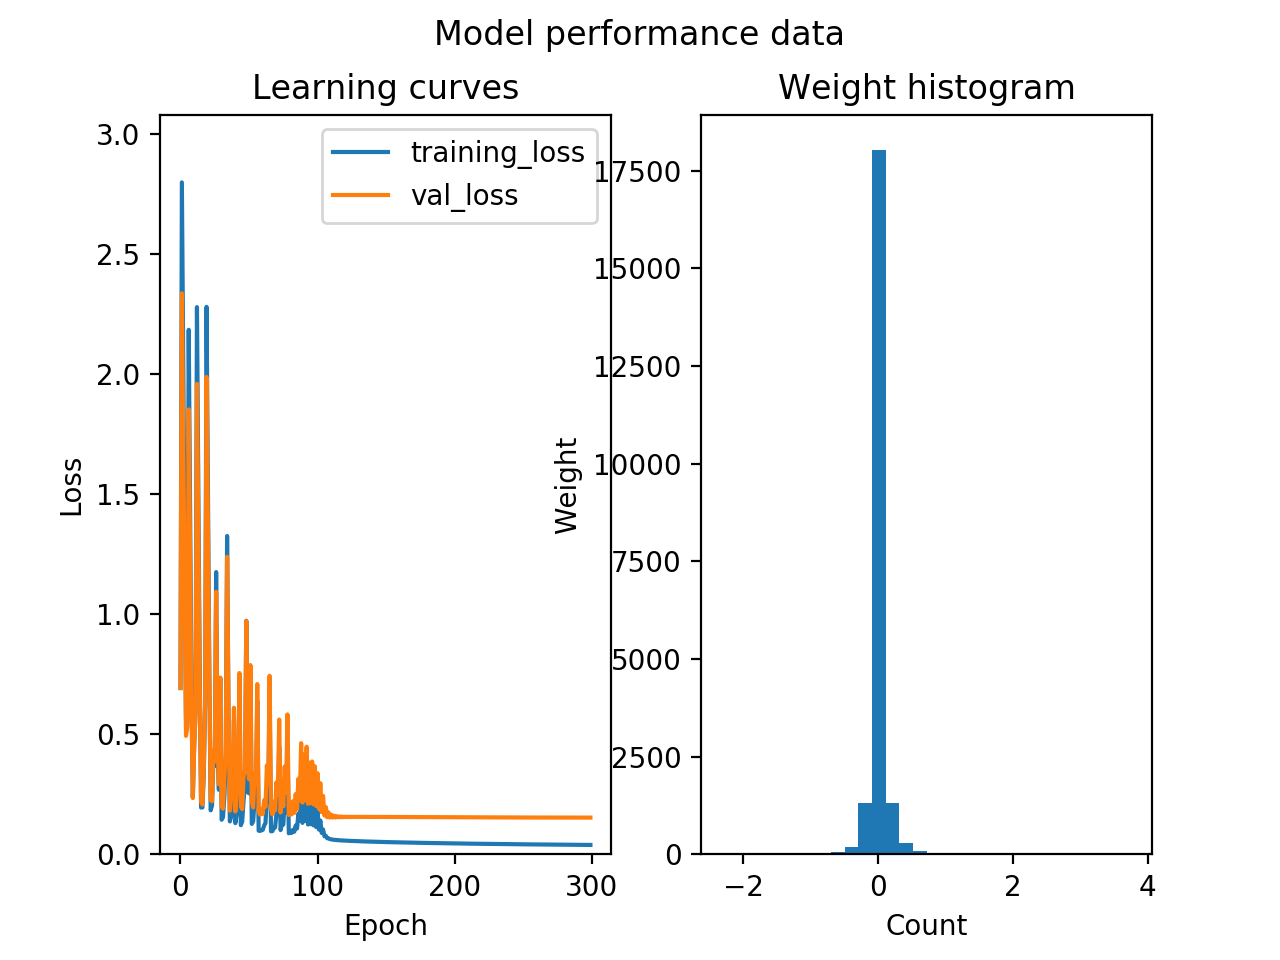
\includegraphics[width=\columnwidth, keepaspectratio]{{../results/12_300_softm_0.0001}.png}
    \caption{Learning Curve Showing High Learning Rate Will Stablize Despite Initial Vibrations}
    \label{fig:learning_rate}
\end{figure}

I also tried to use other loss functions and weight decays. My own logistics loss function worked very similar to the built-in soft margin loss. In fact when the learning rate was low I can get identical scores on both loss funcitons but when the learning rate went up, e.g \verb|learning_rate=3| my logistics performed worse than the soft margin one by 10\%. Other loss functions were worse as well even when running with their best set of hyperparameters. Weight decay can shorten the distance between the training data performance and the validation data one but it didn't help grow the accuracy and the F1 score.

In conclusion, my best set of hyperparameters for now are listed below. They help me achieve 0.937 of accuracy and 0.424 of F1 score on the validation data set.

\begin{lstlisting}[language=Python]
    learning_rate = 12
    epochs = 300
    loss_function = torch.nn.SoftMarginLoss()
    weight_decay = 0.0001
\end{lstlisting}

Both of the top 10 features from the classifier make sense to humans, especially the positive one. Words such as ``stupid'', ``fuck'' and ``dumb'' are clearly signs of discussions went off rail. In the negative features ``='' is the one with lowest weight. In Wikipedia ``='' is used very often in their markup language hence this can be the sign that people are describing a bug or a web page formatting issue rather than the content, which is more rational and less emotional. Other word in the negative features like ``might'', ``Thank'' etc. are typical words in English to express uncertainty (to suggest opposite opinions politely) and grateful.

\subsection{Testing and Reflection}



\end{document}                                                                                                                                                                                  